\section{Absatz- und Zeichenformate}
\href{https://golatex.de/wiki/Kategorie:Befehlsreferenz}{hier geht es zur \LaTeX\ Befehlsreferenz}

\section{Das aktuelle Layout}
\vspace{1cm}
\layout

\section{Umgang mit Anführungszeichen}
Das Setzen beziehungsweise die Verwendung der Anführungszeichen kann am Anfang mit \LaTeX\ ein kleines Problem darstellen.\\
\noindent
«Schweiz» 	\frqq Schweiz\flqq \\
„Deutschland“ und »Deutschland«	  	\glqq Deutschland\grqq{} und \flqq Deutschland\frqq \\
»Österreich« 	\flqq {\"O}sterreich\frqq
%« Frankreich » 	\og Frankreich\fg

\section{Umgang mit Bildern}
Bilder müssen ausserhalb von Tex abgespeichert sein und werden per Referenz eingefügt.

\noindent
\begin{minipage}{1.0\textwidth}
 	\centering
 	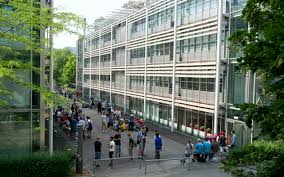
\includegraphics[width=1.0\textwidth]{Kapitel/Bilder/gibbBmSchulhausMitSchuelern}
 	\captionof{figure}{Kein Bild ohne Beschriftung!}
\end{minipage}

Um Bilder nebeneinander zu positionieren hat sich für mich folgendes Vorgehen bewährt. zuerst wird an der Stelle an welcher die Bilder eingefügt werden sollen die Verfügbare Breite "`gemessen"'.

\noindent
ein DIN A4 hat die Dimensionen 210 mm x 297 mm und an dieser Stelle ist die verfügbare Textbreite \convertto{mm}{\the\linewidth} mm.

Danach kopiere ich folgender \LaTeX Code und ersetze die Breite der Bilder (hier auf 70 mm gesetzt). Ich achte darauf, dass beide Bilder zusammen nicht mehr als die angegebene Textbreite - 10mm haben. dadurch ergibt sich ein ungefährer Bildabstand von eben diesen 10 mm. Dadurch ist es ebenfalls möglich bilder mit verschiedenen Grössen zu setzen.

\noindent
\begin{minipage}{0.45\linewidth}
	\centering
	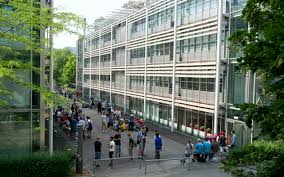
\includegraphics[width=70mm]{Kapitel/Bilder/gibbBmSchulhausMitSchuelern}
	\captionof{figure}{Start zu einer neu zu erstellenden Frage}
	\label{fig:Testbild1}
\end{minipage}\hfill
\begin{minipage}{0.45\linewidth}
	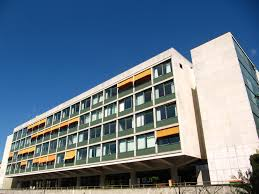
\includegraphics[width=70mm]{Kapitel/Bilder/gibbHauptgebaude}
	\captionof{figure}{Da sollte für jeden Geschmack etwas dabei sein}
	\label{fig:Testbild2}	
\end{minipage}

\section{Umgang mit Code}

\lstset{language=TEX}
Code wir in der speziellen Umgebung \lstinline$\lstlisting$ gesetzt, zum Beispiel: Java \lstset{language=Java} \lstinline$boolean b=true;$ oder Python \lstset{language=Python} \lstinline$sum = float(num1) + float(num2)$ 

mehre Zeilen:
\begin{lstlisting}
if(<boolescher Ausdruck>){
// Anweisung(en)
} else {
// Anweisung(en)
// Anweisung(en)
}
\end{lstlisting}

\newpage
\section{Marginalien}
\leavevmode
\marginpar{margin1}
\marginpar{
\includegraphics[width=1cm]{tex/callouts/achtung.png}}
\marginpar{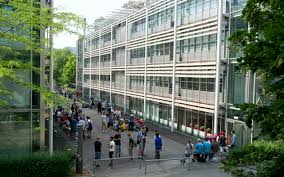
\includegraphics[width=\linewidth]{Kapitel/Bilder/gibbBmSchulhausMitSchuelern}}
Mit der Formatvorlage Marginalie kann ein Absatz in die Marginalien-Spalte links des Haupttexts verschoben werden. Marginalien können bspw. verwendet werden für Anmerkungen, Quellenangaben oder Lizenztexte.
Dabei sind auch Bilder oder kleine Tabellen möglich.
In der Verwendung kann \lstinline$\marginpar{text}$ oder \lstinline$\marginnote{text}$ verwendet werden. Einfach Mal experimentieren \dots

\marginpar{\begin{tabular}{|c|c|}
             \hline 
             1 & 2 \\ \hline
             3 & 4 \\ \hline 
           \end{tabular}
          }
          
\blindtext

\begin{addmargin}[-\marginWidthPlusSep]{0pt}
   	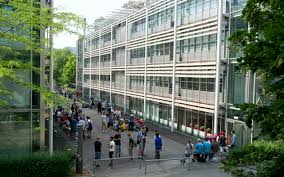
\includegraphics[width=\dimexpr\textwidth+\marginWidthPlusSep]{Kapitel/Bilder/gibbBmSchulhausMitSchuelern}
   	\captionof{figure}{Bild über die ganze Breite ( vorgang funzt auch mit Tabelen\dots)}
   	\label{fig:figur2}    	
\end{addmargin}


\begin{addmargin}[-\marginWidthPlusSep]{0pt}
	\begin{minipage}{60mm}
		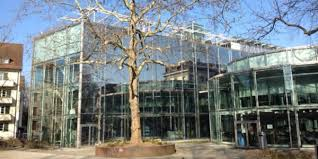
\includegraphics[width=60mm]{Kapitel/Bilder/gibbiet}
		\captionof{figure}{Bild seitlich ausgerückt}
		\label{fig:Testbild3}
	\end{minipage}\hfill
	\begin{minipage}{\dimexpr\textwidth+\marginWidthPlusSep-70mm} % 60mm des Bildes + 10mm abstand
		\blindtext
	\end{minipage}   	
\end{addmargin}

\section{Callouts}

Das Kommando \lstinline$\callout$ setzt wie der name bereits suggeriert ein Callout :-)\\
Verwendung:\\
\lstinline$\callout{picture}{Text}$

\subsection{Achtung}

Dieser Callout wird verwendet um auf besonders wichtige Informationen hinzuweisen.


\callout{achtung}{
	
	Mögliche Werte für \lstinline$picture$

	\begin{itemize}
		\item achtung
		\item arbeitsanweisung
		\item installation
		\item lesen
		\item link
		\item video
		\item weiterfuehrend		
	\end{itemize}
}

\subsection{Arbeitsanweisung}

Dieser Callout wird verwendet um Arbeitsanweisungen hervorzuheben.

\callout{arbeitsanweisung}{Beantworten Sie die Fragen 1–3.}

\subsection{Installation}
Dieser Callout wird verwendet, wenn Schüler Installationsarbeiten vornehmen müssen, bevor sie im Modul weiterfahren können.
	
\callout{installation}{bla bla bla}

\subsection{Lesen}
	
\callout{lesen}{Dieser Callout wird verwendet, um auf externe Literatur zu verweisen.}

\subsection{Link}
Dieser Callout wird verwendet um auf eine Webseite zu verweisen
	
\callout{link}{Dieser Callout wird verwendet um auf eine Webseite zu verweisen. Die ganz mutigen unter uns folgen den Hinweisen auf \href{http://www.gibb.ch}{gibb}. Falls Sie weiter führende Fragen haben so kontaktieren sie die technische \href{mailto:bill.gates@ms.com}{Auskunft} }

\subsection{Video}
Dieser Callout wird verwendet um auf Videos zu verweisen
	
\callout{video}{Bla bla bla. \href{https://youtu.be/ORZYBASS9zw}{cooooles Video} }

\subsection{Weiterführend}
Dieser Callout wird verwendet um auf weiterführende Informationen zu verweisen oder Zusatz- resp. Bonusarbeiten zu kennzeichnen.
	
\callout{weiterfuehrend}{\underline{Achtung:} Das Picture heisst \flqq weiterfuehrend\frqq\ ohne \flqq ü\frqq.}

\subsection{Notiz / Antwortbereich}
Dieses Element wird verwendet für handschriftliche Notizen oder Antworten der Schüler. Das Feld besteht aus einem \flqq multiline Textfield \frqq und kann in seiner Grösse angepasst werden.\\
Verwendung:\\
\lstinline$\antwortbereich{<height>}$

\textbf{Notizen:}\\[0.75ex]
\antwortbereich{100pt}

\blindtext

\newpage
\section{Ausstehende Arbeiten} \label{sec:AusstehendeArbeiten}

\begin{itemize}
	\item Kopfzeile
	\item Die Bilder der Callouts habe ich aus dem Word Dokument als png herauskopiert -> Vermutlich existieren diese aber irgendwo in einer besseren Qualität -> Urs fragen...
	\item 
\end{itemize}


\blindtext[1]

